\documentclass{article}
\usepackage{quantikz}
\begin{document}
\begin{center}
\begin{quantikz}
  \lstick{$\ket{0}$} & \gate{H} & \ctrl{1} & \qw  & \rstick[2]{$\ket{\Phi^+} = \frac{1}{\sqrt{2}}(\ket{00} + \ket{11})$} \\
  \lstick{$\ket{0}$} & \qw      & \targ{}  & \qw  &
\end{quantikz}
\end{center}


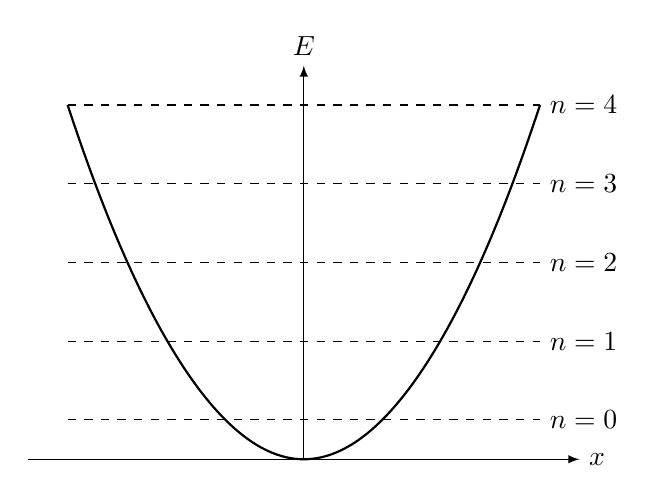
\begin{tikzpicture}[>=latex]
  % Draw axes
  \draw[->] (-3.5,0) -- (3.5,0) node[right] {$x$};
  \draw[->] (0,0) -- (0,5) node[above] {$E$};
  % Draw potential curve V(x) = 1/2 x^2 (parabola)
  \draw[thick] (0,0) parabola (3,4.5);
  \draw[thick] (0,0) parabola (-3,4.5);
  % Draw quantized energy levels E_n = n+0.5
  \draw[dashed] (-3,0.5) -- (3,0.5) node[right] {$n=0$};
  \draw[dashed] (-3,1.5) -- (3,1.5) node[right] {$n=1$};
  \draw[dashed] (-3,2.5) -- (3,2.5) node[right] {$n=2$};
  \draw[dashed] (-3,3.5) -- (3,3.5) node[right] {$n=3$};
  \draw[dashed] (-3,4.5) -- (3,4.5) node[right] {$n=4$};
\end{tikzpicture}


\begin{tikzpicture}[>=latex, line cap=round, line join=round]
  % Axes
  \draw[->] (-3.7,0) -- (3.7,0) node[right] {$x$};
  \draw[->] (0,0) -- (0,5.2) node[above] {$E$};

  % Harmonic oscillator potential V(x) = (1/2) x^2 (in units where ħω=1)
  \draw[thick] (0,0) parabola (3,4.5);
  \draw[thick] (0,0) parabola (-3,4.5);
  \node[anchor=west] at (0.2,4.9) {$V(x)=\tfrac12 m\omega^2 x^2$};

  % Energy levels En = n + 1/2 (units ħω)
  \foreach \n/\E in {0/0.5,1/1.5,2/2.5,3/3.5,4/4.5}{
    \draw[dashed] (-3,\E) -- (3,\E);
    \node[anchor=west] at (3.1,\E) {$n=\n$};
  }
% --- Two particles in the lowest level n=0 ---
  % Place two circles on the n=0 line
  \filldraw[fill=white, thick] (-0.6,0.5) circle (0.12);
  \filldraw[fill=white, thick] ( 0.6,0.5) circle (0.12);

  % Spin arrows: up on left, down on right
  \draw[->, thick] (-0.6,0.53) -- (-0.6,0.85);  % spin up
  \draw[->, thick] ( 0.6,0.85) -- ( 0.6,0.53);  % spin down

  % Optional labels
  \node[anchor=south] at (-0.6,0.88) {$\\uparrow$};
  \node[anchor=north] at ( 0.6,0.50) {$\\downarrow$};

  % Highlight the n=0 level a bit
  \draw[very thick] (-3,0.5) -- (3,0.5);

\end{tikzpicture}



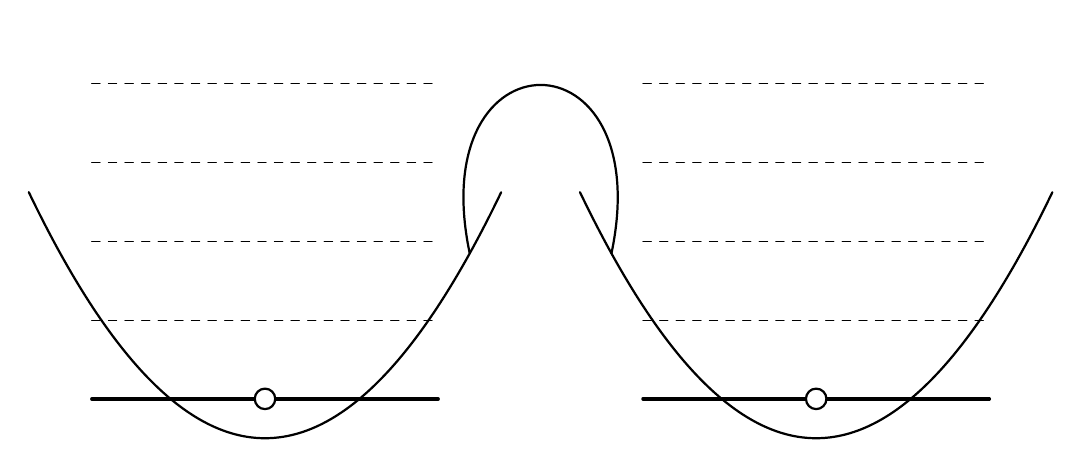
\begin{tikzpicture}[>=latex, line cap=round, line join=round, scale=1.0]

  % ---- Axes (optional) ----
  %\draw[->] (-7,0) -- (7,0) node[right] {$x$};
  %\draw[->] (0,0) -- (0,6) node[above] {$E$};

  % Parameters
  \def\xL{-3.5}      % left well center
  \def\xR{ 3.5}      % right well center
  \def\a{1.2}        % horizontal scale of each parabola
  \def\Emax{4.5}     % top energy level drawn
  \def\yBridge{5.2}  % height of smooth connecting curve on top
  \def\R{0.13}       % particle radius

  % ---- Left harmonic well: V_L(x) = 0.5 * ((x-xL)/a)^2 ----
  \draw[thick, domain=\xL-3:\xL+3, samples=120]
    plot (\x, {0.5*((\x-\xL)/\a)^2});

  % ---- Right harmonic well: V_R(x) = 0.5 * ((x-xR)/a)^2 ----
  \draw[thick, domain=\xR-3:\xR+3, samples=120]
    plot (\x, {0.5*((\x-\xR)/\a)^2});

  % ---- Smooth curve joining the two wells on top ----
  % A smooth arch/bridge drawn as a Bézier curve:
  \draw[thick]
    (\xL+2.6, {0.5*((2.6)/\a)^2})
      .. controls (-1.5, \yBridge) and (1.5, \yBridge) ..
    (\xR-2.6, {0.5*((-2.6)/\a)^2});

  % ---- Energy levels in each well ----
  % (units where ħω=1): E_n = n + 1/2 for n=0..4
  \foreach \n/\E in {0/0.5,1/1.5,2/2.5,3/3.5,4/4.5}{
    % Left levels (short segments inside left well)
    \draw[dashed] (\xL-2.2,\E) -- (\xL+2.2,\E);
    % Right levels (short segments inside right well)
    \draw[dashed] (\xR-2.2,\E) -- (\xR+2.2,\E);
  }

  % Optionally emphasize the n=0 lines
  \draw[very thick] (\xL-2.2,0.5) -- (\xL+2.2,0.5);
  \draw[very thick] (\xR-2.2,0.5) -- (\xR+2.2,0.5);

  % ---- One particle (circle) in lowest level in each well ----
  \filldraw[fill=white, thick] (\xL,0.5) circle (\R);
  \filldraw[fill=white, thick] (\xR,0.5) circle (\R);

  % Optional labels
  %\node[anchor=south] at (\xL,0.5) { };
  %\node[anchor=south] at (\xR,0.5) { };

\end{tikzpicture}



\begin{tikzpicture}[scale=1.0, line cap=round, line join=round]

% Axes (optional)
%\draw[->] (-6,0) -- (6,0) node[right] {$x$};
%\draw[->] (0,0) -- (0,5.5) node[above] {$E$};

% Parameters
\def\a{0.15}    % curvature
\def\b{2.5}     % well separation
\def\Emax{4.5}
\def\R{0.13}

% --- Smooth double-well potential ---
% V(x) = a (x^2 - b^2)^2
\draw[thick, domain=-4.2:4.2, samples=300]
  plot (\x, {\a*(\x*\x-\b*\b)^2});

% --- Energy levels (drawn locally in each well) ---
\foreach \n/\E in {0/0.5,1/1.5,2/2.5,3/3.5}{
  % Left well levels
  \draw[dashed] (-4.0,\E) -- (-1.2,\E);
  % Right well levels
  \draw[dashed] ( 1.2,\E) -- ( 4.0,\E);
}

% Emphasize ground states
\draw[very thick] (-4.0,0.5) -- (-1.2,0.5);
\draw[very thick] ( 1.2,0.5) -- ( 4.0,0.5);

% --- Particles in the ground states ---
\filldraw[white, thick] (-2.5,0.5) circle (\R);
\filldraw[white, thick] ( 2.5,0.5) circle (\R);

% Optional labels
\node[below] at (-2.5,0.3) {$n=0$};
\node[below] at ( 2.5,0.3) {$n=0$};

\end{tikzpicture}


\clearpage


\begin{tikzpicture}[scale=1.0, line cap=round, line join=round]

% -----------------------
% Parameters
% -----------------------
\def\a{0.15}     % curvature of the double well
\def\b{2.5}      % separation of wells
\def\R{0.13}     % particle radius

% -----------------------
% Smooth double-well potential
% V(x) = a (x^2 - b^2)^2
% -----------------------
\draw[thick, domain=-4.2:4.2, samples=300]
  plot (\x, {\a*(\x*\x-\b*\b)^2});

% -----------------------
% Energy levels En = n + 1/2 (ħω = 1 units)
% -----------------------
\foreach \n/\E in {0/0.5,1/1.5,2/2.5,3/3.5}{
  % Left well levels
  \draw[dashed] (-4.0,\E) -- (-1.2,\E);
  % Right well levels
  \draw[dashed] ( 1.2,\E) -- ( 4.0,\E);
}

% Emphasize ground states (n=0)
\draw[very thick] (-4.0,0.5) -- (-1.2,0.5);
\draw[very thick] ( 1.2,0.5) -- ( 4.0,0.5);

% -----------------------
% Particles in ground states
% -----------------------
% Left particle (spin up)
\filldraw[white, thick] (-2.5,0.5) circle (\R);
\draw[->, thick] (-2.5,0.55) -- (-2.5,0.95);
\node[above] at (-2.5,0.95) {$\uparrow$};

% Right particle (spin down)
\filldraw[white, thick] ( 2.5,0.5) circle (\R);
\draw[->, thick] ( 2.5,0.95) -- ( 2.5,0.55);
\node[below] at ( 2.5,0.50) {$\downarrow$};

% -----------------------
% Optional labels
% -----------------------
\node[below] at (-2.5,0.30) {$n=0$};
\node[below] at ( 2.5,0.30) {$n=0$};

\end{tikzpicture}


\begin{tikzpicture}[scale=1.0, line cap=round, line join=round]

% -----------------------
% Parameters
% -----------------------
\def\a{0.15}     % curvature of the double well
\def\b{2.5}      % separation of wells
\def\R{0.13}     % particle radius

% -----------------------
% Smooth double-well potential with softened outer edges
% V(x) = a (x^2 - b^2)^2 * exp(-0.03 x^2)
% -----------------------
\draw[thick, domain=-4.2:4.2, samples=400]
  plot (\x, {\a*(\x*\x-\b*\b)^2 * exp(-0.03*\x*\x)});

% -----------------------
% Energy levels En = n + 1/2  (ħω = 1 units)
% -----------------------
\foreach \n/\E in {0/0.5,1/1.5,2/2.5,3/3.5}{
  % Left well levels
  \draw[dashed] (-4.0,\E) -- (-1.2,\E);
  % Right well levels
  \draw[dashed] ( 1.2,\E) -- ( 4.0,\E);
}

% Emphasize ground states (n = 0)
\draw[very thick] (-4.0,0.5) -- (-1.2,0.5);
\draw[very thick] ( 1.2,0.5) -- ( 4.0,0.5);

% -----------------------
% Particles in ground states
% -----------------------

% Left particle (spin up)
\filldraw[black, thick] (-2.5,0.5) circle (\R);
\draw[->, very thick] (-2.5,0.55) -- (-2.5,1.45);
%\node[above] at (-2.5,1.45) {$\uparrow$};

% Right particle (spin down)
\filldraw[black, thick] ( 2.5,0.5) circle (\R);
\draw[->, very thick] ( 2.5,1.45) -- ( 2.5,0.55);
%\node[below] at ( 2.5,0.45) {$\downarrow$};

% -----------------------
% Optional labels
% -----------------------
\node[below] at (-3.5,0.0) {$n=0$};
\node[below] at ( 3.5,0.0) {$n=0$};

\end{tikzpicture}



\end{document}
